\documentclass{mproj}
\usepackage{graphicx}
\graphicspath{ {./images/} }

\usepackage{url}
\usepackage{fancyvrb}
\usepackage[final]{pdfpages}
\usepackage{times}

\usepackage[newfloat]{minted}
\setminted[python]{fontsize=\footnotesize}


\usepackage{tcolorbox}
\usepackage{caption}

\BeforeBeginEnvironment{minted}{\begin{tcolorbox}[colframe=white!25!white]}%
\AfterEndEnvironment{minted}{\end{tcolorbox}}%

\newenvironment{code}{\captionsetup{type=listing}}{}
\SetupFloatingEnvironment{listing}{name=Code Snippet}

% for alternative page numbering use the following package
% and see documentation for commands
%\usepackage{fancyheadings}


% other potentially useful packages
%\uspackage{amssymb,amsmath}
%\usepackage{url}
%\usepackage{fancyvrb}
%\usepackage[final]{pdfpages}

\begin{document}

%%%%%%%%%%%%%%%%%%%%%%%%%%%%%%%%%%%%%%%%%%%%%%%%%%%%%%%%%%%%%%%%%%%
\title{Source Control Integrated Issue Tracking - The Next Generation of Issue Tracking}
\author{Nystrom Johann Edwards}
\date{7th September, 2018}
\maketitle
%%%%%%%%%%%%%%%%%%%%%%%%%%%%%%%%%%%%%%%%%%%%%%%%%%%%%%%%%%%%%%%%%%%

%%%%%%%%%%%%%%%%%%%%%%%%%%%%%%%%%%%%%%%%%%%%%%%%%%%%%%%%%%%%%%%%%%%
\begin{abstract}
Two areas in which software engineering tools overlap are in issue tracking systems (ITS) and version control systems (VCS). Maintaining both systems is cumbersome and can reduce productivity if focus is constantly switched from developing code to maintaining the issue tracker. This project exemplifies the benefits of combining both tools to reduce the friction between both activities. It shows that the next generation of issue trackers can utilise the power of VCS such that developers can embed issues directly into source code. This combined benefit provides an accurate description of the state of any software project by providing one source of truth. Using the Source Control Integrated Issue Tracking (SCIIT) system we aim to eliminate the friction by extending the VCS and managing issues embedded within the source code. Developers can now update issue information, track development progress, manage collaboration, and inspect complex relationships between their issues and source code as issues are attached to commits.  

Keywords: Issue Tracking, Version Control System, Embedded Issues, Source Code, Git
\end{abstract}

\pagenumbering{roman}
\educationalconsent
\newpage

\section*{Acknowledgements}

I would like to thank my supervisor, Dr Timothy Storer for exposing me to new software engineering possibilities through this project, for his advice and mentoring on creating a new and useful software tool, and most importantly for assistance in making the difficult decisions on design choices.

I would like to thank my wife Virginia for her support and encouragement throughout my programme and all her efforts to ensure that it was completed with great success. I would not have gotten this far without her valuable insight into my projects, her motivational speeches and her uplifting presence.

I am especially grateful to my sister Zophia who has financed my programme and has always believed in supported and encouraged my software development talent. She will always be one of my greatest supporters.

I am grateful to my mother Joslyn and all other members of my family that have invested in my education and encouraged me in this undertaking. Thier efforts will always be greatly appreciated.

Finally, I would like to thank my colleagues at the university that helped in the evaluation of the project that provided feedback needed to make a good solution.

%%%%%%%%%%%%%%%%%%%%%%%%%%%%%%%%%%%%%%%%%%%%%%%%%%%%%%%%%%%%%%%%%%%
\tableofcontents




%%%%%%%%%%%%%%%%%%%%%%%%%%%%%%%%%%%%%%%%%%%%%%%%%%%%%%%%%%%%%%%%%%%
\chapter{Introduction}\label{intro}

\pagenumbering{arabic}
\section{Background}

\section{The Problem}

\section{Objectives}

\section{Contribution}

\section{Structure}

%Present state of the art software project issue tracking tools, such as GitHub, GitLab, and JIRA store issues in a database alongside the version control repository that contains the project's source code. This creates friction in development efforts because software developers must remember to keep both the issue tracker and the version control repository up to date as progress is made on completing tasks.

There are many tools used by software engineers in order to create high quality, high performance and maintainable software products. These tools are used by various levels within an organisation in order to coordinate efforts to this end. As such, they are exposed to a wide range of persons collaborating to meet this goal.

Issue tracking systems is at the fore front of collaborating tools when it comes to software development. Bertram (2010) argues that it is used by various groups of persons in order to have a common point of knowledge when it comes to the product that is being developed \cite{Bertram:2010}. For developers in particular the issue tracking system is used as a means to store information on development tasks. Tasks may include, the development of a new feature, the discovery of a bug, the preparation for a release, among others. When progress is made on these tasks it is recorded in the tracker and it provides key information to managers and the team what has taken place.

Version control systems by comparison allow for a similar type of collaboration, however at its core it is the working progress of the entire development of the software product. Here we see the overlap of the two systems where one is related to the product as a working growing artifact and the other as a planning and knowledge base on segments of the software product. Integrating the two systems would potentially provide the benefit of keeping track of both types of critical information in a format that does not duplicate work efforts.

We propose to introduce developers to an extension of the version control system that allows for the tracking of issues as a first step in testing this theory. It is expected that a tool such as this will allow developers to remain highly collaborative on issues and productive on writing code into version control thereby reducing the friction of maintaining two systems and switching focus during development.

%%%%%%%%%%%%%%%%%%%%%%%%%%%%%%%%%%%%%%%%%%%%%%%%%%%%%%%%%%%%%%%%%%%
\chapter{Analysis}\label{analysis}

\section{Related Work}

\section{Related Products}

\section{Key Concerns}
%%%%%%%%%%%%%%%%%%%%%%%%%%%%%%%%%%%%%%%%%%%%%%%%%%%%%%%%%%%%%%%%%%%
\chapter{Design and Implementation}\label{design}

%talk about git and how we intent to extend its functionality

Git the open source VCS was used as the backbone of the new system. As the most popular open source VCS  technology to date, it offers the opportunity to attain vast amounts of information on its internal mechanisims in order to extend it to include custom functionalities such as an issue tracker. The documentation of Git and the wide variety of related products, articles and examples gives insight into how it is extended. In this project one extension option of Git called Git hooks is specifically utilised. Additionally, an open source python library is utilised to interact with the Git objects and manipulate Git commands. Finally, various interfaces we required to view and manage the issue tracker information. These three mechanisims allowed building a unique system that integrates ITS with VCS.

% talk about how we embed issues into the source code

The first step of integrating issue tracking into a version control system such as Git is a way to store issues alongside commits. This is achieved by embedding the issue and its related information into the source code of the software project files as a block comment in that source code's language structure. The mandatory requirement for embedding and issue is to provide an issue id using an \textbf{\textit{@issue}} flag. Whereas all other information can be optional or supplied in later commits. After a commit is made the SCIIT system then extracts the embedded issue information from files that have been changed during this commit and stores it within its own repository with its object references. The following is an example of an embedded issue:

\begin{code}
\captionof{listing}{Example of an embbed issue in python}
\begin{minted}{python}
"""
    @issue signin
    @title Create a signin page
    @description
      Create a signin page for users of the website. 
      Include social signin and terms and conditions acceptance.
    @assigned to nystrome, kevin, daniels
    @due date 12 Oct 2018
    @label design, ui
    @weight 6
    @priority high    
"""
\end{minted}
\end{code}

% describe how git stores revisions

%In order to achieve such a task, embedded issues are extracted from the source code revisions in the VCS. 
In Git revisions, files are stored as a compressed versions of the entire file and its contents called blobs. When new revisions (additions, modification and deletions) to files are found, Git saves the compressed blobs to its objects directory and creates a new reference by hashing the blob's contents. These references are known as \textit{sha} references. To keeps track of the blobs, references to them are assigned to trees which may represent the folder containing the blob or the root folder of the project.  The root folder tree is then in turn referenced to the commit. This way every commit made represents the full state of the software project during development. The series of references from blobs to trees and trees to commits are the main mechanism for identifying revisions in the VCS. To determine the files that were changed it is now just a matter of comparing new hashes of file contents to the corresponding older references.

% describe its effect on the development of sciit

The integrated issue tracker SCIIT follows the same principle of using references however, they are assigned to objects in a different manner. When a commit is created, the system reads the changes to the source code in that commit and identifies the existence of embedded issues. The contents or information of the embebbed issue is extracted and used to form its reference. All the issues identified are then cached to the file system for quicker access as compressed file objects. All the issue references that were identified beloning to that commit are then collectively assigned to an issue tree. Unlike Git, SCIIT contains just one issue tree per commit. This keeps the SCIIT disk space usage on the file system as small as possible since the creation of may file objects add disk space overheads. Consequentially, any commits that do not contain issues point to the same empty issue tree object. Additionally, any issues that have not been changed over time are continually referenced on to the next commit.

\begin{figure}[t]
\caption{SCIIT ITS to VCS Filesystem Design}
\label{fig:sciit-filesystem}
\centering
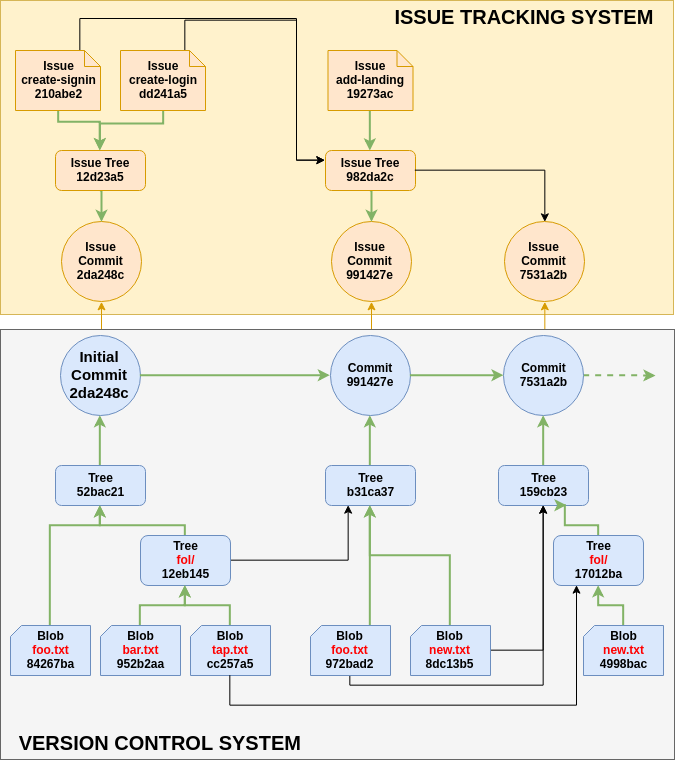
\includegraphics[width=10cm]{sciit-filesystem}
\end{figure}

% describe how issues are stored and managed

Each individual issue tree reference is attached to a special object called an issue commit. For all intents and purposes, they contain the reference to a Git commit and a reference to an issue tree. This way they represent both the ITS and VCS creating one system that manages both activities. The resulting Source Control Integrated Issue Tracking (SCIIT) System can now be adequately used to represent the complex relationships between the management of issues and the state of the software project. Figure \ref{fig:sciit-filesystem} shows how SCIIT integrates the ITS alonside the VCS on the file system as a series references when commits are created.

As shown in Figure \ref{fig:sciit-filesystem} every commit made in Git generates an issue commit that contains references to all the revisions made to those issues. This therefore poses a change in the traditional management of issues. If an issue is changed by editing the issue data embedded in the soruce code as a comment then a new issue object is created and assigned to a new issue tree. Changes to the references of an issue object over time can now be associated with a change in the issue. The issue tracker also intuitively determines if issues are closed by removing references to an issue that has been deleted from the embedded comment.

% how it works in a distributed environment

\section{Distributed Integration}

It is worth pointing out some design considerations of the system operation in a distributed environment since the backbone of the system is based on a distributed VCS. In Git, the main object of concern when it comes to a distributed environment is the branch. Each user has a local copy of the entire source code. They can make there changes locally and then push it to a remote repository where it can be merged with changes by other developers. In order to achieve such workflows branches are used. They represent a deviation from references to commits on other branches. Each branch has a HEAD which is a reference to the latest commit made on that branch. This way commits can now have different parents depending on which branch they belong to.

Although branching and merging, pushing and pulling are the main mechanisims allowing for distributed VCS, they all are based on the same primative object, the commit. Since our issue tracker was based on this primative object, a branch from a commit will contain issue commits, issue trees and issues which may differ from other branches. This allows them to contain branch specific issues. The utility of this design allows for the issue tracker to also be distributed in the sense that some issues can only be referenced from particular branches.

This concept gets compounded in merging senarios. In such events, developers can now be alerted by the VCS that there is a conflict with the issues as the full file contents of both referenced files are compared. At this point developer team members can decide in their merges or code reviews whether sufficient work has been done on the issue, if the issue is closed appropriately, or if to add more details in the issue for future development work. At merge points the primative commit object is saved with parent references to more than one prior commit. The SCIIT system will again scan this commit for embedded issues and update the issue tracker references.

\begin{figure}[t]
\caption{Distributed Issue Tracking}
\label{fig:distributed-issue-tracking}
\centering
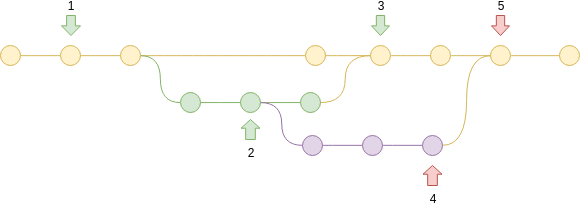
\includegraphics[width=10cm]{distributed-issue-tracking}
\end{figure}

Figure \ref{fig:distributed-issue-tracking} shows how this is achieved. At point 1 a new issue is added for the first time into the orange branch. Commits that follow this keep the reference the to issue created here until a user modifies the embedded issue information or removes it from the source code. When branching to green, issue 1 remains open in both branches. At point 2 another issue is created. Here there are two issues open on the green branch and one open on the orange. The purple branch inherits both issues from the green branch. At point 3, developers make the decision to merge issue 2 into the orange branch. At point 4, both issue 1 and 2 are closed by deleting the embedding from the source code. Here there are no issues on the purple branch. At point 5, developers decide that the work has actually been completed and resolves the merge conflict by deleting the two issue embeddings from the source code. This shows the distributred nature of issues.

%%%%%%%%%%%%%%%%%%%%%%%%%%%%%%%%%%%%%%%%%%%%%%%%%%%%%%%%%%%%%%%%%%%%%%%%%%

\section{Mechanisms and Architecture}

% talk about the git python library and how we intend to use this library to interface with the git objects in python
    % how the library was extended
    % 

\subsection{GitPython}

In order to implement such a system it must be able to read information from the Git repository and to create issue tracking objects referenced to each commit. GitPython an open source python library is extended for this purpose and one of the three main mechanisms of SCIIT. Objects in the library that are related directly to the repository are extended to provide the extra functionality needed for managing issues. Two objects in particular are extended; the Repository object which allows for manipulating the Git repository and the Objects object allows for manipulating the raw Git objects (commits, trees, and blobs). Added to these objects were the ability to manipulate issues, issue trees, issue commits, and the issue repository.

% integrating git with sciit allows for the inference of many pieces of information required by issue trackers

\subsection{Git Hooks}

Git hooks are the second main mechanism that allows for the handling of issues. In this project three hooks in particular are utilised; the post-commit, post-merge, and post-checkout. The post-commit hook comminicates with the SCIIT library in order to search for embeddings and create issues in the ITS for every commit made. This hook reduces the friction of the programmer having to switch focus to the issue tracker at this point to update issue information or status. Just one activity is required to do both. The post-merge hook is utilised during two Git events; merging and pulling. In order for SCIIT to be useful to teams, the issues that other developers create must be syncronised between all members of the team. When pulling down the VCS from the remote repository, SCIIT will then build the issue objects for the difference of commits on the local machine and the remote. This allows all on the team to collaborate on the same issues. Similarly, during a merge, the repository is syncronised to ensure that all commits have the correct issue references. The post-checkout hook is similar to the merge in that it syncronises issue references with commits. This is particularly implemented for the users that just fetch Git commits from the remote to checkout at a later stage.

\subsection{Interfaces}

The last main mechanism of the SCIIT system is its interface channels. There are three interface channels that provide three different services. 

The first is a command line interface. The CLI does not allow for direct manipulation of issues but it allows for users to refresh the issue repository, view individual issues and view issue tracker. The initialisation commmand creates the issue repository and builds issue objects from past commits. This is essential for Git since developers can work on software projects that already exist. The developers can clone a project and then initialise the issue tracker by building all the issue references that were embedded in the commits. Initialisation also sets up the Git hooks required for the project to be able to track new issues. 

There is a command for viewing the tracker. This allows for user to see the status of all issues in the issue tracker. It also shows the complex relationships between the ITS and VCS such as participants, creator, commit activities to the issue, changes in description and revisions to the issue over time. This command shows the power of integrating ITS and VCS such that complex relationships can be inferred from the issue and version control repository objects. It also allows for showing the state of the issue tracker between revisions of commits that may be on different branches. Futher CLI commands and its uses can be found in Appendex B Figure \ref{fig:sciit-cheatsheet} or screenshoots of the issue tracker can be found in % Appendix C Figure \ref{fig:sciit-tracker-shot1}.

The second is a web interface. This interface shows the issue tracker to the user by lauching a local web browser with all the issue tracking information loaded into html view. Users are not allowed to edit any of the information within this interface but it gives and easier display for users to view their issues, read through issue activity and view all other inferred data which performing developing tasks.

The thrid is an intermediate webservice that allows for the integration of GitLab issues with the SCIIT System. The main reason for having such an interface is that it allows for non developer members of a project such as coaches, team leads, production staff or contributors to create issues in GitLab that will create commits with embedded issues. This module was developed to show that SCIIT and its principles could be integrated with traditional ITS to engage non developer users. The webservice works by using GitLab Webhooks in conjuction with SCIIT on a webserver and the GitLab API as follows:

\begin{itemize}
  \item \textbf{Push Webhooks:} These hooks are triggered when developers push commits to the repository. A HTTP request is then sent to the SCIIT webservice interface. The interface then fetches the changes from the GitLab remote repository as a mirror repository and syncs the Git commits with the ITS issue references. Any new references that are made during this revision are then packaged and requests are made to the GitLab Issues API to create or edit those issues. Commit actitvity during this revision are added to the GitLab issue as notes.
  \item \textbf{Issue Webhooks:} These hooks are triggered when someone creates or edits an issue in the GitLab web interface. A HTTP request is then sent to the SCIIT webservice interface. The interface then takes the issue title and issue description that was changed and makes changes to the relevant source code contents of the file that corresponds to the issue. If it has not been assigned to a file previously a new file is created to track the new issue. It then makes a request to the GitLab Commits API to create a new commit with the specified changes.
\end{itemize}

When this webservice is attached to the GitLab remote repository, it syncs GitLab issues, SCIIT issues and commits such that the developer need not be concerned that the issues they create or need to work on is not in the SCIIT system. A simple pull from the remote repository will bring in the related commits and refresh the issue tracker and its details.

\subsection{Software Architecture}

Figure \ref{fig:sciit-software-arch} shows the software architecture of SCIIT. There are two seperate file system storage at the heart. One responsible solely for the VCS information and the other for issues. The VCS information is accessed by the higher level tool Git which in term can be manipulated by the GitPython Library. The SCIIT Library has direct access to the issue repository and is responsible for managing all the objects stored within that context. Git hooks allow for the Git application to call on functions of the SCIIT Library when commit, merge, pull and checkout events take place. All combined these components make up the SCIIT system which allows for the manipulation of VCS and ITS objects.


\begin{figure}[t]
\caption{SCIIT Software Architecture}
\label{fig:sciit-software-arch}
\centering
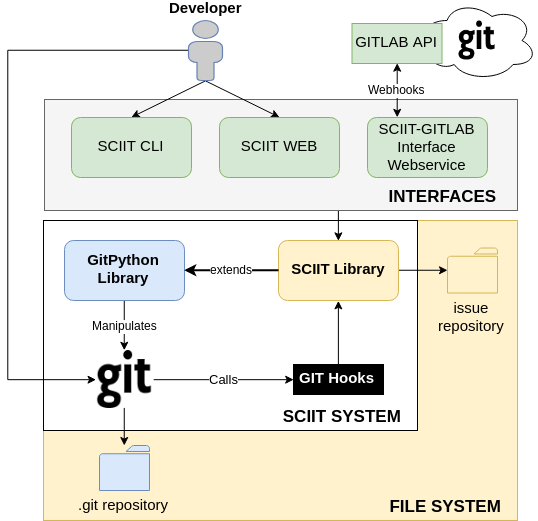
\includegraphics[width=10cm]{sciit-software-arch}
\end{figure}
% talk about the cli used to access the issues after they are created


%As previously discussed in the chapter on design, the issues are cached to the file system. In order to get the issue tracking information out of these object we must build the tracker from 






\section{Challenges}

Since the SCIIT system is first of its kind there would be some challenges associated with its design and development. The following outlines the major design and development challenges
% build time

The first major challenge concerns Git as a light weight system that invloves single threaded file access operations. When building the issue repository from past commits, SCIIT traverses each file object scans its contents to determine if an issue is persent or not. This is a time consuming process and can only be preformed in a single thread. If multiple threads, we will encounter I/O errors, especially since there is a high likelihood that the same file may be accessed or open in many threads. This limits the performance of SCITT to build issues from past commits on repositories that consist of a high number of commits such as the Linux Open Source Project or Tensorflow. Also the performace also suffers based on the commit/merge strategy that the developer teams are using since some strategies can have commits that contain a larger tree of file changes that other strategies. This is the major challenge of the project and its design based on Git. See Appendix A on Perfomance Issues

% communicating with webservice
The second major challenge concerns the use of GitLab API calls within the webservice interface. GitLab Webhooks are a part of the main functionality of the website. For example, utilising the GitLab Commits API triggers a Push Webhook. As such, during development special care needed to be taken to verify the dates of receiving GitLab webhooks with the internal webservice time. If a Webhook was triggered and came in within seconds of another they would be ignored as it would have originated from API calls within the webservice. In our webservice handling Issue Hooks generated requests for handling Push Hook and vice versa. If this was not carefully handled internally then the webservice would be in an infinate loop creating GitLab Issues and commit on the repository.

\section{Summary}

This chapter shows the design of a Source Code Integrated Issue Tracker and how it can be developed to utilise the power of both ITS and VCS. The benefit of which is to allow developers to focus on what they know and deal with the best which is source code. They are now less burdened with the resposibility of diligently maintaining an ITS as all the issues are now embedded into the VCS revisions. This should now reduce the friction between maintaining and issue tracker and developing code as the activities are combined and automated. The next chapter will discuss the impact that such a system will have on the developer, developer teams, and project activities.

%%%%%%%%%%%%%%%%%%%%%%%%%%%%%%%%%%%%%%%%%%%%%%%%%%%%%%%%%%%%%%%%%%%
\chapter{Evaluation}\label{evaluation}


% These three hooks ensure that the ITS issues stays in reference to the VCS commits. It also shows that the end user does not need to be concerend about

%for eval section ==>> In a traditional sense however, issue trackers are meant to be a centralised system. Also if we consider that work is being done on a branch we should be able to capture all the information for all issues on all branches without conflicting data. Fortunately, Git also allows for the querying of revisions such that all commits on all branches are returned maintaing thier parental links. The next chapter describes how this was implemented in order to maintain the valuable issue information on all branches.


% highlight the benefits achieved by the design

%for eval section ==>> By maintaining issues in this manner we can see that a significant step has been taken to reduce the friction between the two development activities of maintaining the ITS and VCS. Developer now need only concern themselves with pulling, and pushing code to the repository where the issue tracker will seemlessly build, track and maintain issues in the background. This does not mean that developers are not resposible for looking at the embedded issues and performing the task it requires to implement them. However, it allows them to work in an environment with one point of contact. The design of SCIIT allows for developers to trod along writing code and to care for the issue tracking process. Additionally the issue tracker will now be up to date with the state of each revision of the source code.

\section{Testing}


%%%%%%%%%%%%%%%%%%%%%%%%%%%%%%%%%%%%%%%%%%%%%%%%%%%%%%%%%%%%%%%%%%%
\chapter{Conclusion}\label{conclusion}

\section{Future Work}

\appendix % first appendix
%%%%%%%%%%%%%%%%%%%%%%%%%%%%%%%%%%%%%%%%%%%%%%%%%%%%%%%%%%%%%%%%%%%
\chapter{Performance Issues}


%%%%%%%%%%%%%%%%%%%%%%%%%%%%%%%%%%%%%%%%%%%%%%%%%%%%%%%%%%%%%%%%%%%
\chapter{Additional Diagrams}
\begin{figure}[h!]
\caption{SCIIT Command Line Interface Cheatsheet}
\label{fig:sciit-cheatsheet}
\centering
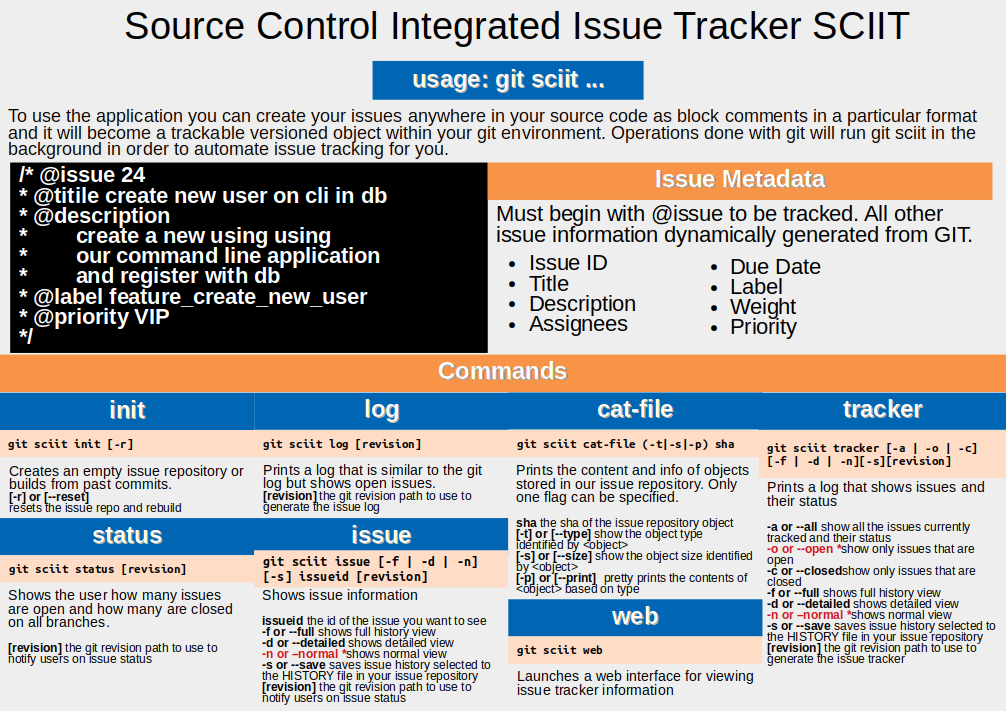
\includegraphics[width=16cm]{Cheatsheet}
\end{figure}

%consider making a diagram for the sciit webservice

%%%%%%%%%%%%%%%%%%%%%%%%%%%%%%%%%%%%%%%%%%%%%%%%%%%%%%%%%%%%%%%%%%%%
\chapter{Screenshots}





%%%%%%%%%%%%%%%%%%%%%%%%%%%%%%%%%%%%%%%%%%%%%%%%%%%%%%%%%%%%%%%%%%%%
\chapter{Development Strategy}



%%%%%%%%%%%%%%%%%%%%%%%%%%%%%%%%%%%%%%%%%%%%%%%%%%%%%%%%%%%%%%%%%%%
% it is fine to change the bibliography style if you want
\bibliographystyle{plain}
\bibliography{mproj}
\end{document}
